\section{Alternatives to Likelihood Computation}
The approximate histograms constitute a new set of inputs for CovEst.
With an ambition to make CovEst more precise and more robust to the approximation inaccuracies,
we would like to alter CovEst to better cope with the inacuraccies produced by
Kmerlight or KmerGenie.

As we show in \ref{sec:estimation-variance}, we can estimate the variance and 
model the disribution of Kmerlight's errors. We noticed that different histogram columns $f_i$
have different variances and so we want to incorporate these differences into CovEst.

When CovEst searches for the most likely parameters $\theta$, it evaluates the likelihood
of the observed histogram by comparing $\hat f_1, \hat f_2, \dots, \hat f_m$ and 
$p_1, p_2, \dots p_m$. The idea of the improvement is to provide the variances of 
$\hat f_i$ as an additional input to CovEst. With these variances, CovEst could
attribute higher importance to the columns with lower variance and attribute
lower importance the the columns with value $\hat f_i$ fluctuating more.

Let us denote the exact histogram as $f$ and the observed approximated histogram as $\hat f$.
CovEst should seek the shape of histogram $f$ by maximizing $P(\hat f \,|\, f)$. 

\subsection{KmerGenie's Errors}
\label{sec:kmergenie-errors}
In \ref{sec:simple-sampling} we described a method used by KmerGenie to compute 
an approximate histogram. In this section we provide a simple analysis of KmerGenie's
errors that will in turn help us understand the relationship of Kmerlight's histograms
and CovEst.

Each distinct $k$-mer is either counted by KmerGenie with probability $1/s$ or it is discarded 
with probability $1 - 1/s$. Therefore, the abundance of a $k$-mer does not change 
with sampling process -- either all of its occurences are counted or none of them are.
This means that the estimate $\hat f_i$ is computed only from those $f_i$ distinct $k$-mers 
that contribute to the column $f_i$ by having abundance $i$. No other $k$-mers can
influence the value $\hat f_i$.

On average $f_i / s$ $k$-mers with abundance $i$ are chosen and counted by KmerGenie.
Moreover, the number of these $k$-mers follow a binomial distribution $Bin(f_i, 1/s)$
and it holds for the estimates that
$$\hat f_i \sim s \cdot Bin(f_i, 1/s)$$
The random vector $(\hat f_1, \hat f_2, \dots, \hat f_m, d)$, where $d$ is a number
of distinct discarded $k$-mers follows a multinomial distribution 
$$s \cdot Mult\left(F_0, \frac{f_1}{F_0} \frac{1}{s}, \frac{f_2}{F_0} \frac{1}{s}, \dots, 
\frac{f_m}{F_0} \frac{1}{s}, 1-\frac{1}{s}\right)$$
that can be interpreted as putting $F_0$ $k$-mers into $m+1$ buckets. With this knowledge we can
calculate the probability $P(\hat f\,|\,f)$.

\medskip

How to incorporate this knowledge into CovEst? We can notice that, in fact, to maximize 
$P(\hat f\,|\,f)$ it is sufficient to find $\arg \max_f \left(\sum_{i=1}^m \hat f_i \log f_i
\right)$. And this is exactly the same expression as the one maximized by CovEst 
(\ref{eq:covest-likelihood}).

Here we find that CovEst by design expects the inaccuracies produced by KmerGenie
and thus there is no space for improvement.




\subsection{Likelihood Function for Kmerlight}
In section \ref{sec:estimation-variance} we approximated the distribution of Kmerlight
estimates with normal distribution and therefore
we first tried to modifiy CovEst with the new likelihood computation formula 
$\sum_{i=1}^m \log g(\hat f_i;\, p_i \cdot \hat F_0, \sigma_i^2)$. The term $g(x; \mu, \sigma^2)$  
denotes the probability density of the normal distribution at value $x$. This formula depitcts the
log-likelihood of observing $m$ independent variables $\hat f_i$ that come from $m$
normal distributions.

As a proof of concept, we calculated the sample variance of $\hat f_i$ from 50 observations 
and we provided these variances as additional input for CovEst.
Unfortunately, it often happened that the value $p_i \cdot \hat F_0$ guessed by CovEst was distant
from the observed value $\hat f_i$ and thus the probability density was extremely low for these
columns. As a result, the log-likelihood of CovEst's initial guess reached \texttt{-infinty} 
and so CovEst was unable to optimize parameters $\theta$. The estimates $\hat c$ 
were thus very inaccurate.

\medskip

To theoretically estimate Kmerlight's variance we used the concept of sampling from $k$-mers in 
\ref{sec:estimation-variance}. We assumed that Kmerlight counts each $k$-mer with probability 
$p_s$ and discards each $k$-mer with probability $1 - p_s$. In other words, we approximated 
the Kmerlight's process with exactly the same process as KmerGenie uses. 

Later in \ref{sec:estimation-variance} we included the effect of medians by multiplying the 
variance by a constant (and by using the normal distribution instead of binomial) 
and in \ref{sec:variance-experiments} we showed that these assumptions lead to a good 
approximation of the distribution of Kmerlight's estimates.

The important thing to notice is that the errors of Kmerlight can be modelled in a very similar 
way to the errors of KmerGenie. As the binomial distribution converges to the normal distribution 
with increasing amount of data, the shapes of Kmerlight and KmerGenies distributions are similar.
Moreover, for both Kmerlight and KmerGenie the variance of $\hat f_i$ increases linearly with 
$f_i$. For Kmerlight it can be seen from (\ref{eq:variance}) and for KmerGenie it can be seen 
from the variance of binomial distribution ($np(1-p)$ for $Bin(n,p)$). 

Since Kmerlight's errors distribution is similar to KmerGenie's distribution
and since CovEst is designed to expect this type of error distribution,
we can conclude that CovEst is also robust with respect to Kmerlight.




\subsection{Minimizing the Sum of Square Errors}
The inspiration to minimize the weighted sum of square errors comes from the work of
Williams et al. \cite{Williams2013}. In their paper the authors present a generative probabilistic
model similar to CovEst, but instead of maximizing the probability $P(\hat f\,|\,f)$ they
minimize
\begin{equation} \label{eq:wminsq}
\sum_{i=1}^m \frac{1}{\hat f_i}(\hat f_i - f_i)^2
\end{equation}
where $\hat f$ is the observed histogram and $f$ is a guessed histogram.

We compared the method used by CovEst (\ref{eq:covest-likelihood}) to the method
based on minimizing the square errors (\ref{eq:wminsq}) on multiple exact and approximated
histograms and we conclude that both methods result in equally precise estimates.

\medskip

The advantage of the method (\ref{eq:wminsq}) over the method based on log-likelihood
is that it is easy to incorporate different variances for different $i$ into
the minimization formula as weights. As we would like the columns with higher
variance to have lower impact, we can divide each square
error by the variance and we get the following formula 
$\sum_{i=1}^m \frac{1}{\sigma^2_i}(\hat f_i - f_i)^2$, where $\sigma_i^2$ denotes the variance
of the $i$-th column. 

For Kmerlight and KmerGenie, $\sigma_i^2 \propto f_i$ and therefore (\ref{eq:wminsq}) 
is also robust with respect to Kmerlight's and KmerGenie's errors and we were not able
to achieve more accurate estimates than the estimates produced by CovEst originally. 
If the character of errors was different, however,
this approch might lead to a more precise estimates.

\medskip

To test whether we can improve CovEst's accuracy with this approach on some inputs, we generated 
histograms with a different variance profile. 

We first generated a genome and reads as described in \ref{sec:data-generation} and then we computed
the exact histogram with Jellyfish. We set $\sigma_i = f_i$, thus the variance increases
proportionally to $f_i^2$, instead of $f_i$. Then we simulated the histogram approximation by
modifying the exact histogram. In each of 100 trials we generated a histogram $\hat f$
that consisted of $\hat f_i \sim N(f_i, f_i^2), \hat f_i \geq 0$.

In Figure \ref{img:covest-alternative} we present boxplots of coverage estimation errors.
The estimates produced with use of weighed sum of square errors have lower variance
than the estimates produced with use of log-likelihood maximization.

\begin{figure}[h]
\hspace{-0.3cm}
\centerline{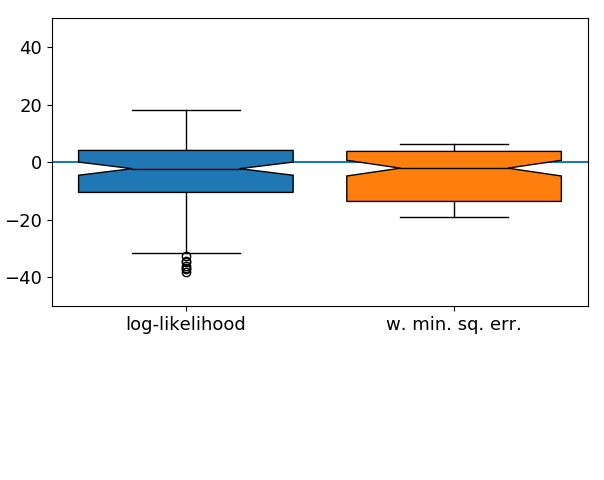
\includegraphics[width=0.7\textwidth, trim={0cm, 3.5cm, 0cm, 0cm}, clip]{{images/covest_alternative_boxplot}.png}}
\caption[CovEst estimates with different histogram comparison methods]{Distributions of coverage 
estimate errors with two different methods used in CovEst's parameter optimization --
maximizing the log-likelihood (blue), minimizing the sum of weighed of square errors (orange).}
\label{img:covest-alternative}
\end{figure}
